\chapter{Uma Ontologia para Experimentos em LPS (SMartOntology)}
\label{sec:ontologia}

Este tópico apresenta conceitos fundamentais sobre a proposta de ontologia SMartyOntology. Inicialmente foi realizado um processo de concepção do modelo em seguida foi desenvolvido o projeto desenvolvido se obter modelo. Com a finalidade de avaliação foi desenvolvido um exemplo de aplicação por meio de uma predição de recomendação qual artefato de LPS pode ser usado por um dado templete de experimento. Ao final desse capitulo foi realizado uma avaliação empírica do modelo, por meio de uma ferramenta que avalia pontos de falha do modelo.

\section{Concepção}
\label{sec:concepcao}

Com base na tipologia proposta por \cite{almeida2003visao} definimos o tipo de ontologia proposto na Tabela \ref{tab:type_ontology}:

\begin{table}[]
	\caption{Type of the Proposed Ontology}
	\label{tab:type_ontology}
	\begin{tabular}{@{}lll@{}}
		\toprule
		Approach & Rating & Description \\ \midrule
		\begin{tabular}[c]{@{}l@{}}As for the Mizoguchi function; \\ Vanwelkenbuyse; Ikeda (1995)\end{tabular} & \begin{tabular}[c]{@{}l@{}}Domain ontologies\end{tabular} & \begin{tabular}[c]{@{}l@{}}Reusable in the domain, they provide vocabulary \\ about concepts and their relationships, about the \\ activities and rules that govern them\end{tabular} \\
		\begin{tabular}[c]{@{}l@{}}As for the degree of Uschold formalism; \\ Gruninger (1996)\end{tabular} & Semi-formal & \begin{tabular}[c]{@{}l@{}}Expressed in natural language in a restricted \\ and structured way\end{tabular} \\
		\begin{tabular}[c]{@{}l@{}}As for the Jasper application; \\ Uschold (1999)\end{tabular} & \begin{tabular}[c]{@{}l@{}}Ontologies as specification\end{tabular} & \begin{tabular}[c]{@{}l@{}}An ontology is created for a domain, which is used \\ for documentation and maintenance in the \\ development of software.\end{tabular} \\
		\begin{tabular}[c]{@{}l@{}}As for the Haav structure; \\ Lubi (2001)\end{tabular} & \begin{tabular}[c]{@{}l@{}}Domain ontologies\end{tabular} & \begin{tabular}[c]{@{}l@{}}Describe vocabulary related to a domain, \\ such as medicine or automobiles\end{tabular} \\
		\begin{tabular}[c]{@{}l@{}}As for Van-Heijist content; \\ Schreiber; Wielinga (2002)\end{tabular} & \begin{tabular}[c]{@{}l@{}}Knowledge modeling ontologies\end{tabular} & \begin{tabular}[c]{@{}l@{}}Specify knowledge conceptualizations, have a \\ semantically rich internal structure, and are refined \\ for use in the domain of knowledge they describe\end{tabular} \\
		& \begin{tabular}[c]{@{}l@{}}Application ontologies\end{tabular} & \begin{tabular}[c]{@{}l@{}}Contains the definitions needed to model knowledge\\ in an application\end{tabular} \\
		& \begin{tabular}[c]{@{}l@{}}Domain ontologies\end{tabular} & \begin{tabular}[c]{@{}l@{}}Express concepts that are specific to a \\ given domain of knowledge\end{tabular} \\ \bottomrule
	\end{tabular}
\end{table}

Ou seja, quanto à função é uma ontologia de domínio, quanto ao grau de formalismo é uma ontologia semi formal, quanto à aplicação é uma ontologia de especificação, quanto à estrutura é uma ontologia de domínio e quanto ao conteúdo é tanto uma ontologia para modelagem de conhecimento quanto para aplicação e de domínio.

Foi aplicado o seguinte processo de elaboração da ontologia \cite{fernanda2007modelagem}:

\begin{itemize}
	\item Definição e estruturação dos termos por meio de classes;  
	\item Estabelecimento de propriedades (atributos) inerentes ao conceito representado por um termo;
	\item Povoamento da estrutura que satisfaçam um conceito e as suas propriedades;  
	\item Estabelecimento de relações entre os conceitos;
	\item Elaboração de sentenças para restringir inferências de conhecimento baseadas na estrutura.
\end{itemize}

Inicialmente foi desenvolvido um grafo para o modelo inicial da ontologia SMartyOntology, principalmente para validar os termos por meio de classes, subclasses e os relacionamento entre elas.

\begin{figure}[ht]
	\centering 
	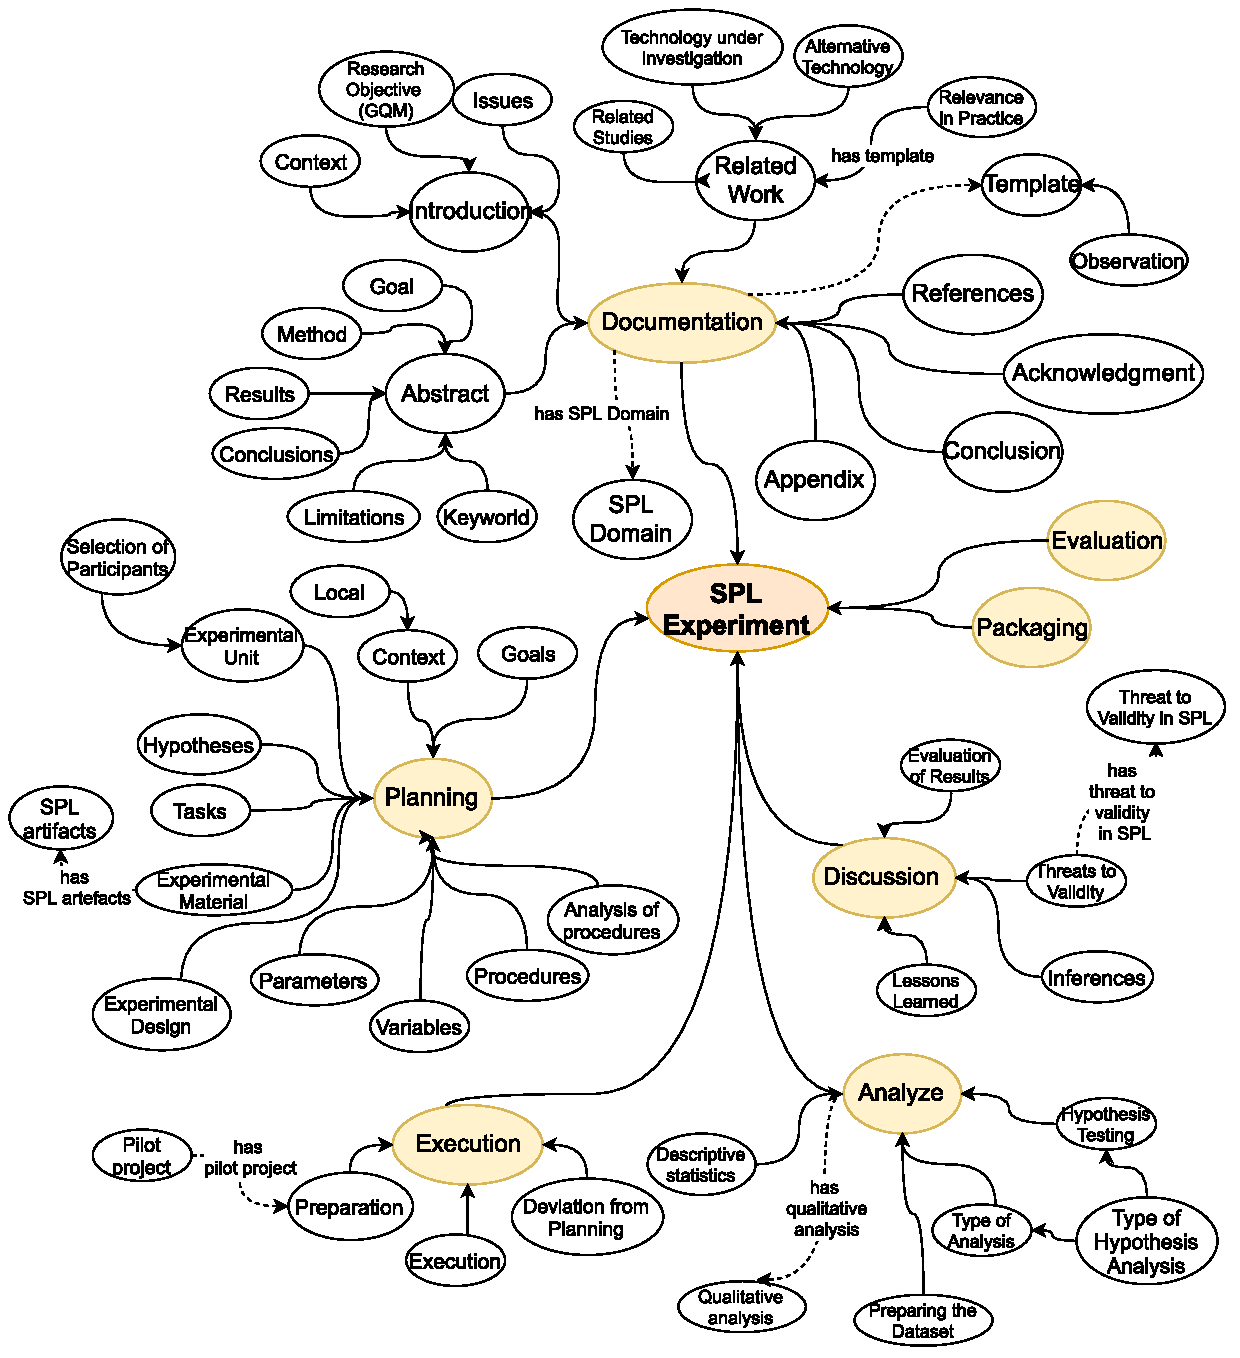
\includegraphics[width=11cm]{graph-all-class.pdf}
	\caption{Initial graph of ontology.}
	\label{figure:graph-all-class}
\end{figure}

A \ref{figure:graph-all-class} representa este modelo inicial contendo a definição principal das classe de mais alto nível para o experimento, SPL Experiment, Documentation, Template, Evaluation, Discussion, Analysis, Execution e Planning. Em seguida evoluímos para possíveis subclasses delas, onde definimos as sub-classes em \ref{tab:class_sub_class_ontology}:

\begin{table}[]
	\caption{Classes and Sub-classes of ontology prototype}
	\label{tab:class_sub_class_ontology}
	\begin{tabular}{@{}lll@{}}
		\toprule
		Class & Sub-class & Sub-class \\ \midrule
		\multirow{19}{*}{Documentation} & \multirow{6}{*}{Abstract} & Keyword \\
		&  & Limitations \\
		&  & Conclusions \\
		&  & Results \\
		&  & Method \\
		&  & Goal \\
		& \multirow{3}{*}{Introduction} & Context \\
		&  & Research Objective \\ & & (GQM) \\
		&  & Issue Issues \\
		& \multirow{4}{*}{Related Work} & Related Studies \\
		&  & Technology under \\ & & Investigation \\
		&  & Alternative Technology \\
		&  & Relevance in Practice \\
		& Template & Observation \\
		& References &  \\
		& Acknowledgment &  \\
		& Conclusion &  \\
		& Appendix &  \\
		& SPL Domain &  \\
		\multirow{11}{*}{Planning} & Context & Local \\
		& Experimental Unit & Selection of Participants \\
		& Experimental Material & SPL artifacts \\
		& Experimental Design &  \\
		& Goals &  \\
		& Hypotheses &  \\
		& Tasks &  \\
		& Parameters &  \\
		& Variables &  \\
		& Procedures &  \\
		& Analysis of procedures &  \\
		\multirow{3}{*}{Execution} & Preparation &  \\
		& Execution & Pilot \\
		& Deviation from Planning &  \\
		Analyze & Type of Analysis & Type of Hypothesis \\ & & Analysis \\
		& Hypothesis Testing &  \\
		& Descriptive statistics &  \\
		& Qualitative analysis &  \\
		& Preparing the Dataset &  \\
		Discussion & Threats to Validity & Threat to Validity \\ & & in SPL \\
		& Evaluation of Results &  \\
		& Inferences &  \\
		&  &  \\
		Packaging &  &  \\
		Evaluation &  &  \\ \bottomrule
	\end{tabular}
\end{table}

A criação deste modelo inicial de ontologia se baseada no trabalho de mapeamento sistemático de experimentos em SPL \cite{Furtado2018}, por meio de uma análise exploratória dos dados levantados nesse mapeamento. O mapeamento servir como guia de informações e metadados de experimentos.

O mapeamento sistemático se baseou no temple experimental de Wohlin, que traz 5 pilares para elaboração de ESE, são eles: Definição, Planejamento, Operação, Análise e Interpretação \cite{wohlin2012}.

\begin{figure}[htb]
	\centering 
	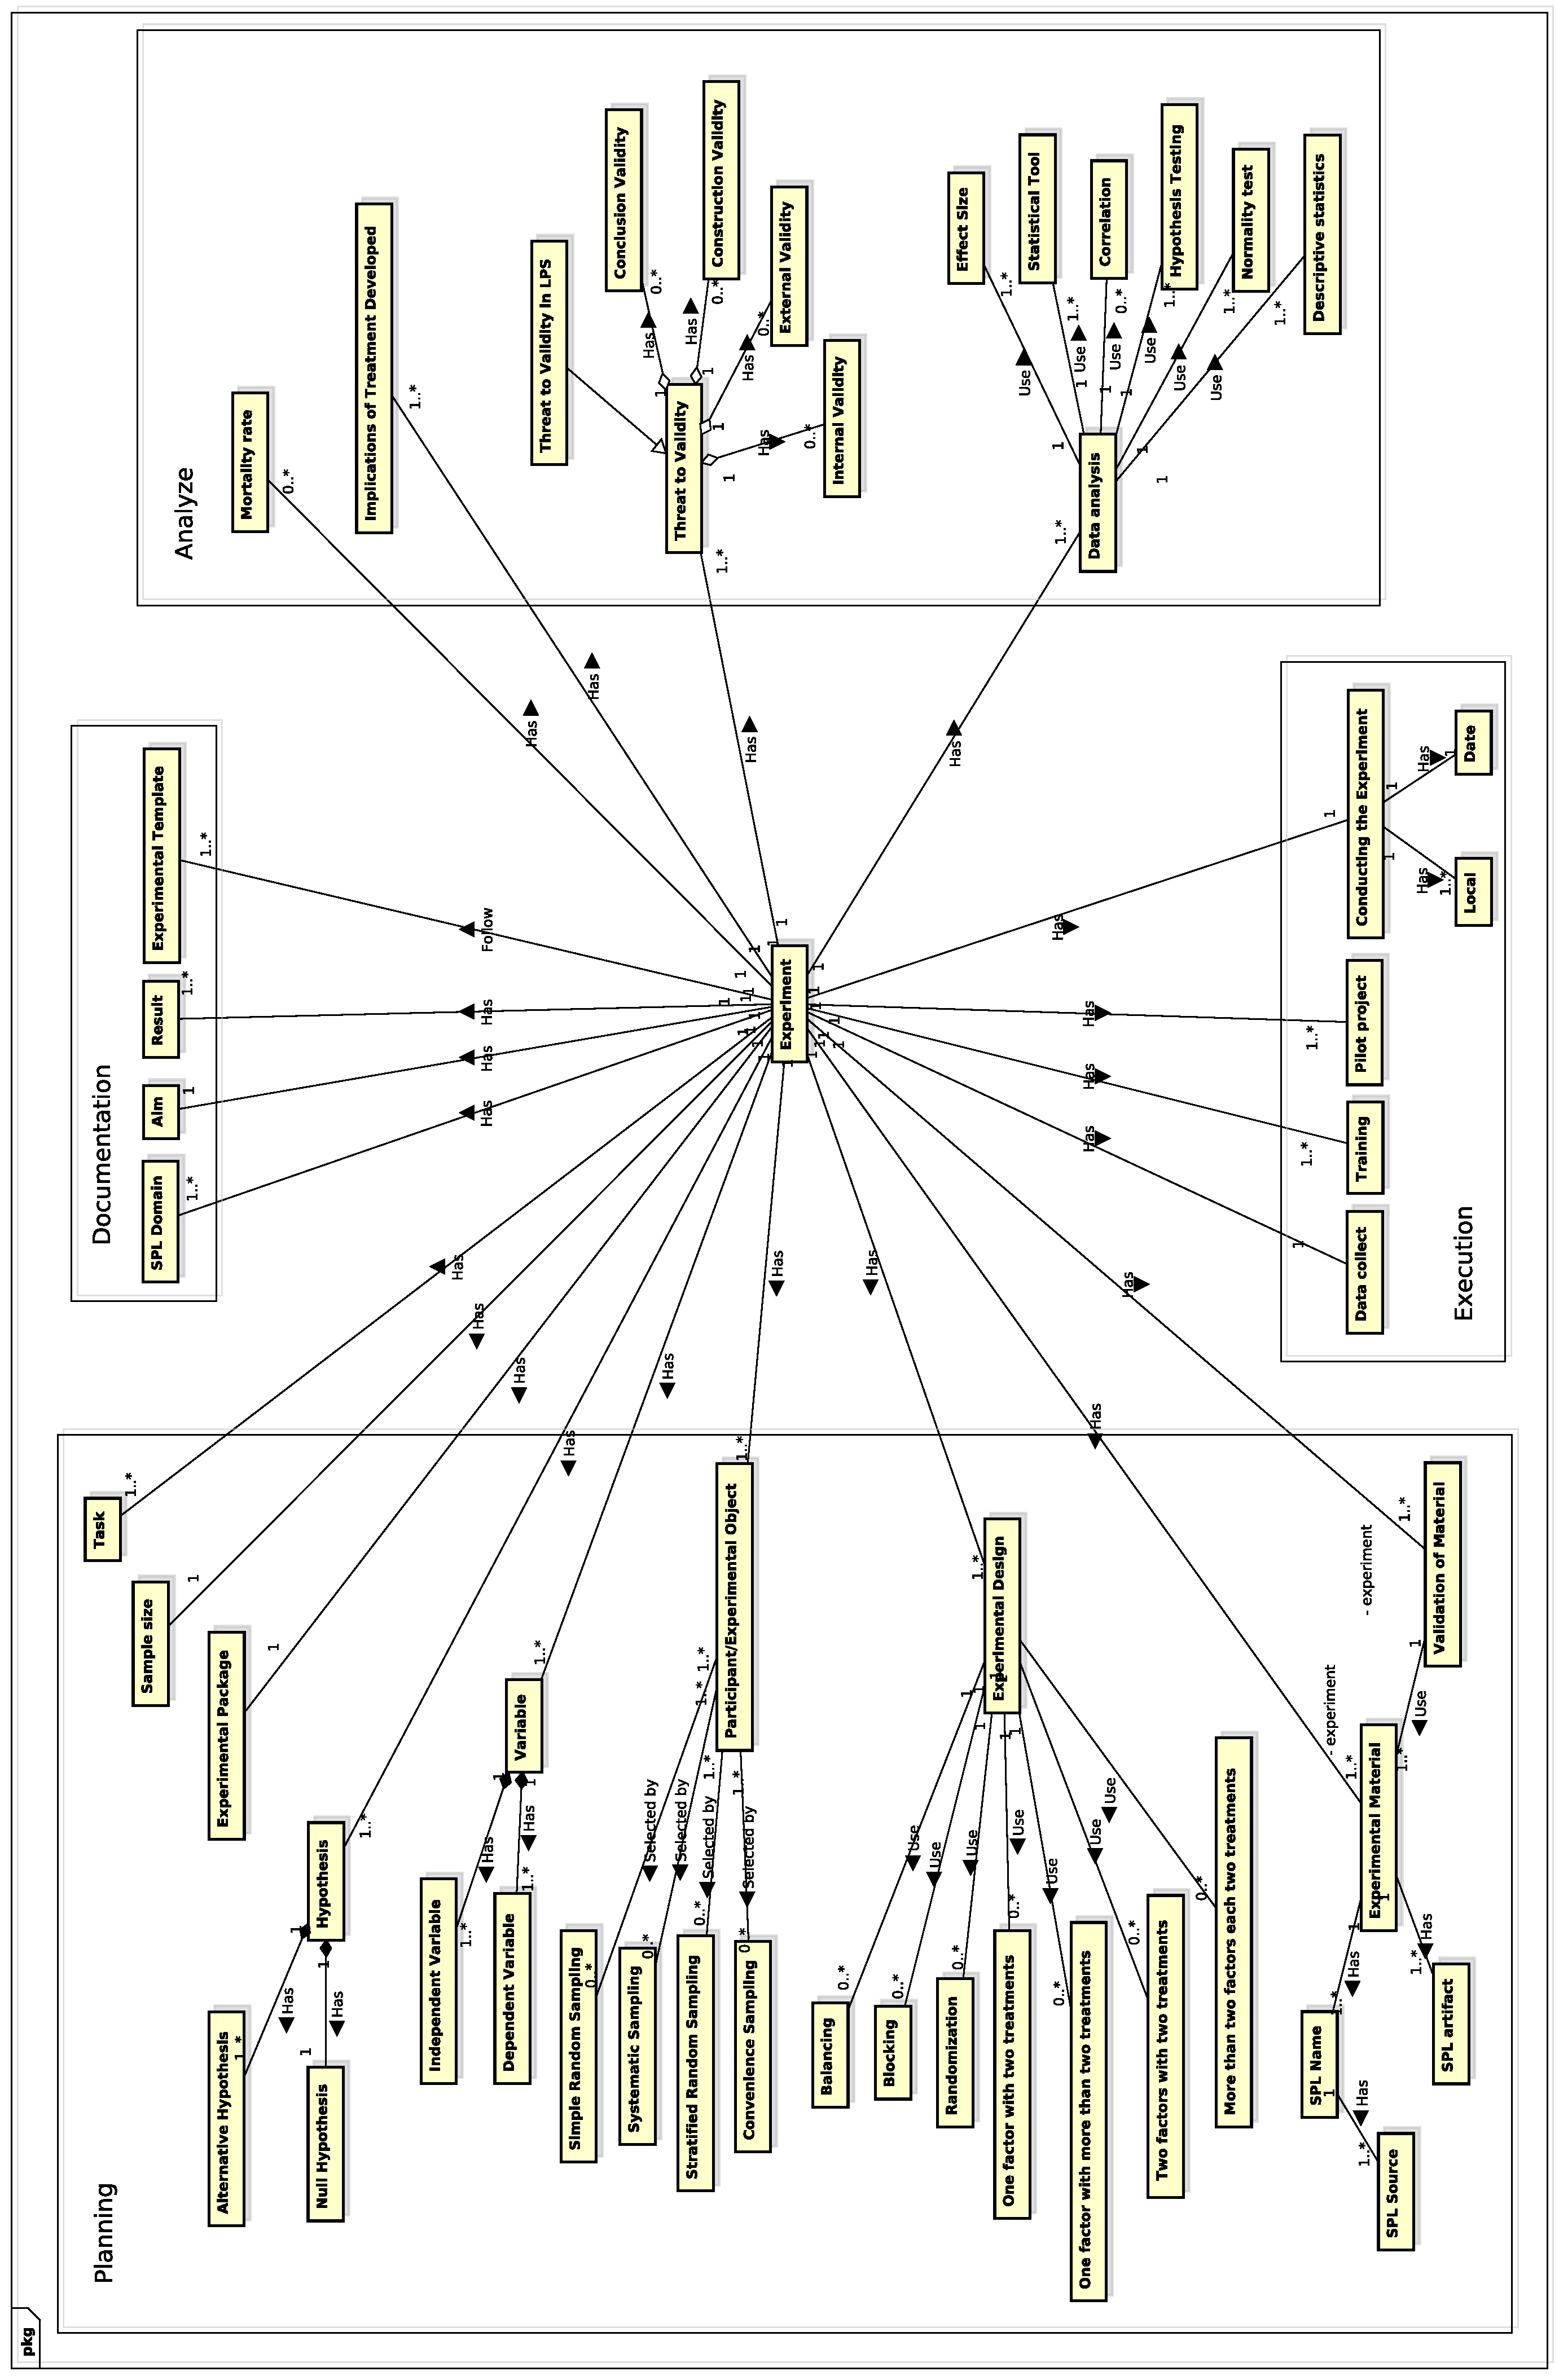
\includegraphics[scale=.2]{conceptual-model-clustering.pdf}
	\caption{Conceptual Model Clustering.}
	\label{figure:conceptual_model_clustering}
\end{figure}

A \ref{figure:conceptual_model_clustering}, apresenta uma modificação do modelo conceitual original, aplicando uma clusterização baseada nos pilares do Wohlin. Esta clusterização foi necessária para compreensão mais abstrata das relações entre os termos do domínio levantados no modelo conceitual original. Dessa forma foi possível validar as classes pai do grafo inicialmente proposto.
	
Em seguida, um diagrama de classes foi criado para uma representação mais formal da modelagem inicial. Nessa representação, a relação entre os termos (classes) e suas propriedades (atributos) ficou mais clara, o modelo TBox. Essa forma de representação destacou a relação principal quando definimos a composição da classe Experiment e ExperimentSPL em quase todas as outras subclasses. Nesta representação também foi explícita a tipificação das propriedades, modelo ABox.

\begin{figure}[htb]
	\centering
	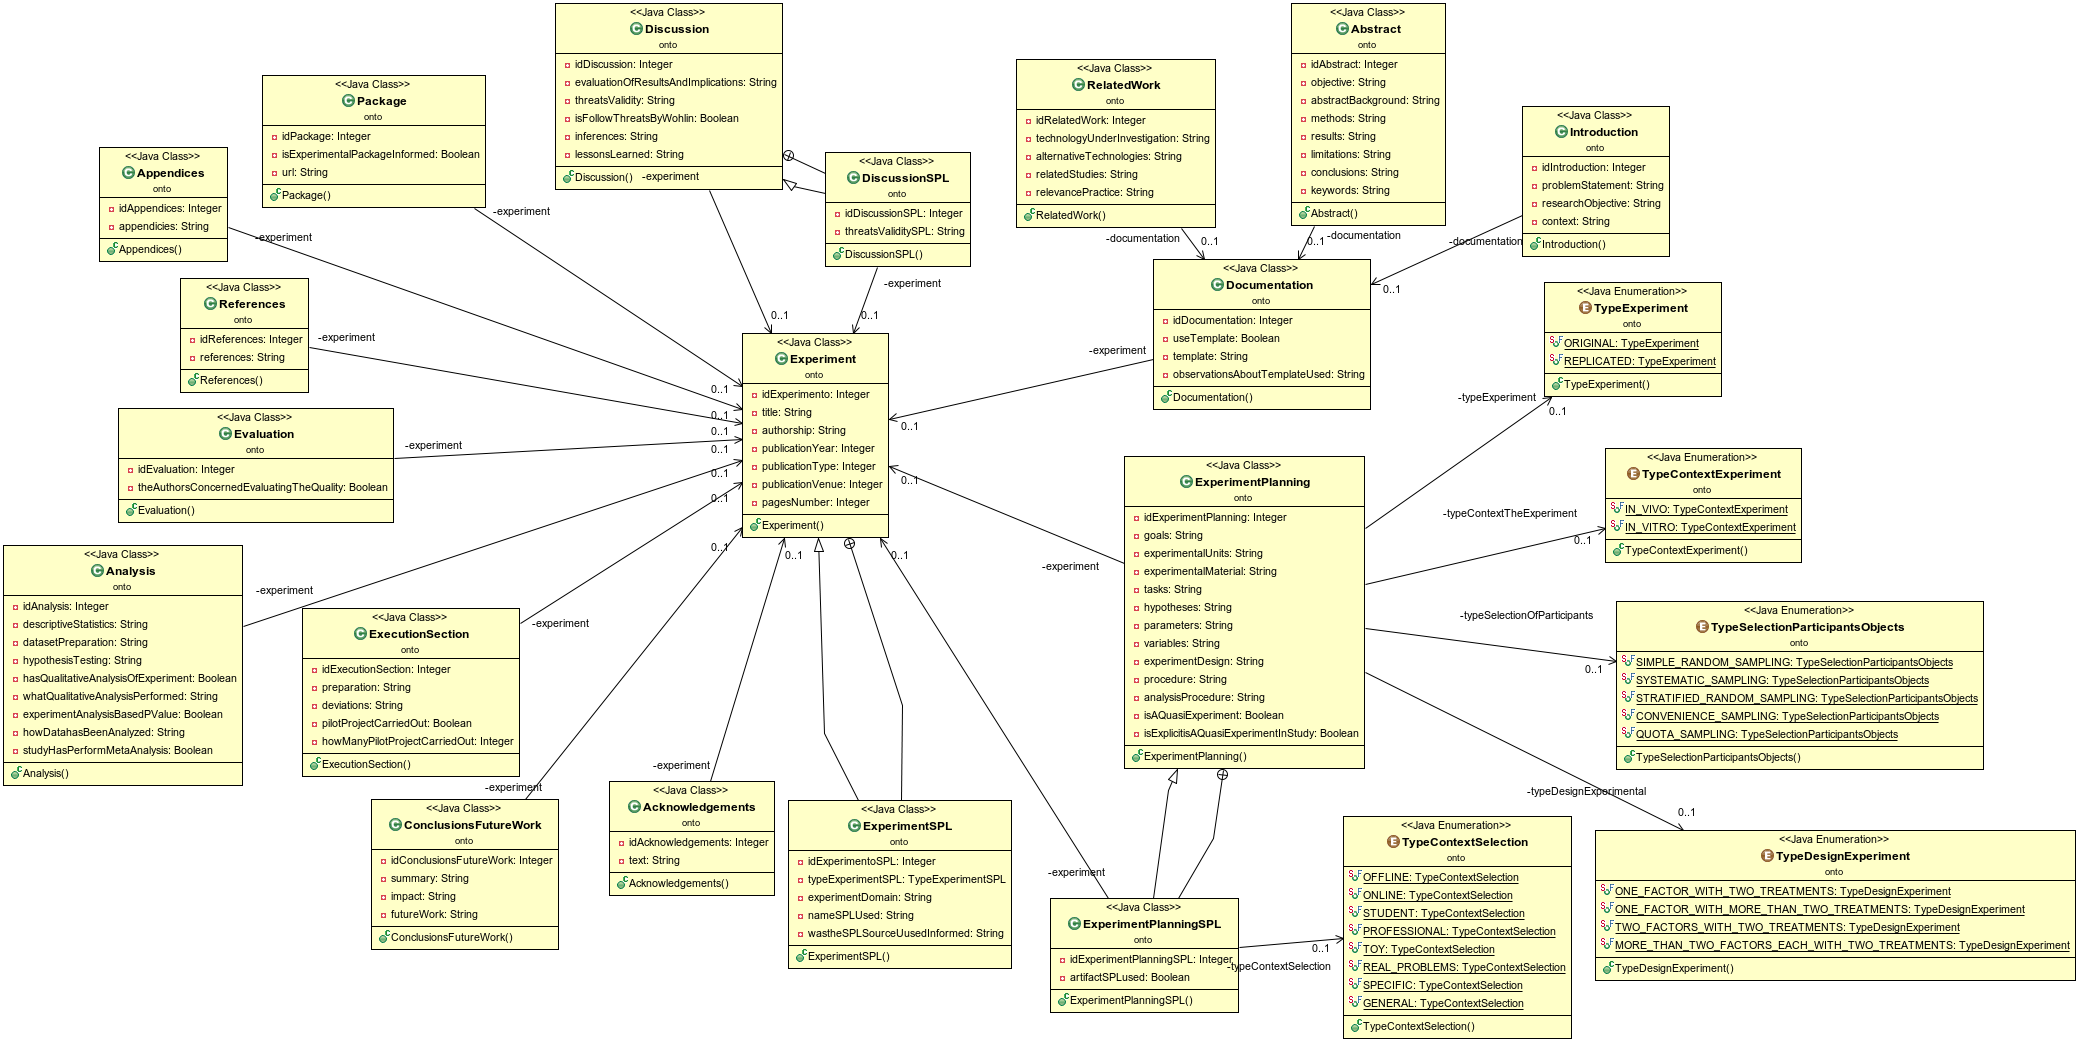
\includegraphics[scale=.2]{class-diagram-ontology.png}
	\caption{Class Diagram for proposal of the ontology model.}
	\label{figure:class_diagram_ontology}
\end{figure}

A \ref{figure:class_diagram_ontology} apresenta  diagrama de classe gerado para SMartyOntology.

Posteriormente, definimos usar a ferramenta Protégé para a construção oficial da ontologia. Esta ferramenta dispõe de uma interface gráfica para edição de ontologias e uma arquitetura para a criação de ferramentas baseadas em conhecimento. Pode ser usada tanto por desenvolvedores de sistema como por especialistas em domínio para criar bases de conhecimento, permitindo representar facilmente o conhecimento de uma área. Este editor é capaz de tratar classes, com sua definição e exemplos, simultaneamente \cite{DBLP:journals/aimatters/Musen15}.


\section{Projeto}
\label{sec:projeto}

Definimos a criação da ontologia usando OWL construindo as classes e subclasses para representar os elementos da ontologia.

\subsection{Protegé}
\label{sec:protege}

O padrão OWL foi usado no SMartyOntology para definir todos os elementos, classes e subclasses.

Fazendo uma analogia ao diagrama de classe, no Protégé, classes, os atributos de classes e seus relacionamentos estão em um contexto de entidades. As classes e hierarquias são definidos na aba Class, os relacionamentos são definidos na aba Propriedades de Objetos e os atributos são definidos na aba Propriedade dos Dados.

Definimos nossas entidades com base do diagrama de classe construído na fase de concepção, com a seguinte estrutura (i) definição de classes (ii) definição das propriedades de objetos, (iii) definição das propriedades dos dados.

\begin{table}[htbp]
	\caption{Ontology Design - Classes and Properties modeling}
	\label{tab:ontology_design_classes_properties}
	\centering
	\begin{tabu} to \textwidth {| p{1.4cm} | p{15.6cm} |}
		\hline
		\centering \textbf{Element} & \centering \textbf{Definition} \\ \hline
		
		Classes & Abstract, Acknowledgments, Analysis, Appendices, ConclusionsFutureWork, Discussion, DiscussionSPL, Documentation, Evaluation, ExecutionSection, Experiment, ExperimentSPL, ExperimentPlanning, ExperimentPlanningSPL, Introduction, Package, References, RelatatedWork, TypeContextExperiment, TypeContextSelection, TypeDesignExperiment, TypeEsperiment, TypeEsperimentSPL, TypeSelectioParticipantObjects \\ \hline
		
		Object Properties & documentation, experiment, typeContextxperiment, typeContextSelection, typeDesignExperiment, typeExperiment, typeExperimentSPL, typeSelectionOfParticipants \\ \hline
		
		Data \mbox{Properties} & idExperiment, title, authorship, publicationYear, publicationType, publicationVenue, pagesNumber, idExperimentSPL, nameSPLUsed, wasTheSPLSourceUsedInformed, idDocumentation, useTemplate, template, observationsAboutTemplateUsed, idAbstract, objective, abstractBackground, methods, results, limitations, conclusions, keywords, idIntroduction, problemStatement, researchObjective, context, idRelatedWork, technologyUnderInvestigation, alternativeTechnologies, relatedStudies, relevancePractice, idConclusionsFutureWork, summary, impact, futureWork, idExperimentPlanning, goals, experimentalUnits, experimentalMaterial, tasks, hypotheses, parameters, variables, experimentDesign, procedureProcedure, explicitQuesiExperimentInStudy, isAQuasiExperiment, idExperimentPlanningSPL, artifactSPLused, idExecutionSection, preparation, deviations, pilotProjectCarriedOut, howManyPilotProjectCarriedOut, idAnalysis, descriptiveStatistics, datasetPreparation, hyp othesisTesting, whatQualitativeAnalysisPerformed, howDatahasBeenAnalyzed, experimentAnalysisBasedPValue, hasQualitativeAnalysisOfExperiment, studyHasPerformMetaAnalysis, idDiscussion, evaluationOfResultsAndImplications, inferences, lessonsLearned, threatsValidity, isFollowThreatsByWohlin, idDiscussionSPL, threatsValiditySPL, idAcknowledgements, acknowledgments, idReferences, references, idAppendices, appendicies, idEvaluation, theAuthorsConcernedEvaluatingTheQuality, idPackage, isExperimentalPackageInformed, url, isLinkAvailable \\ \hline
	\end{tabu}
\end{table}

\subsubsection{Definição de classes}
No Protégé, definimos uma classe raiz chamada Thing na qual todas as outras classes são filhas dela. A \ref{figure:class_defition_protege} apresenta a definição da classe Experiment dentro do modelo, neste momento a definição é composta pelo nome da classe e seus principais relacionamentos (Equivalent To e SubClass Of).

\begin{figure}[]
	\centering 
	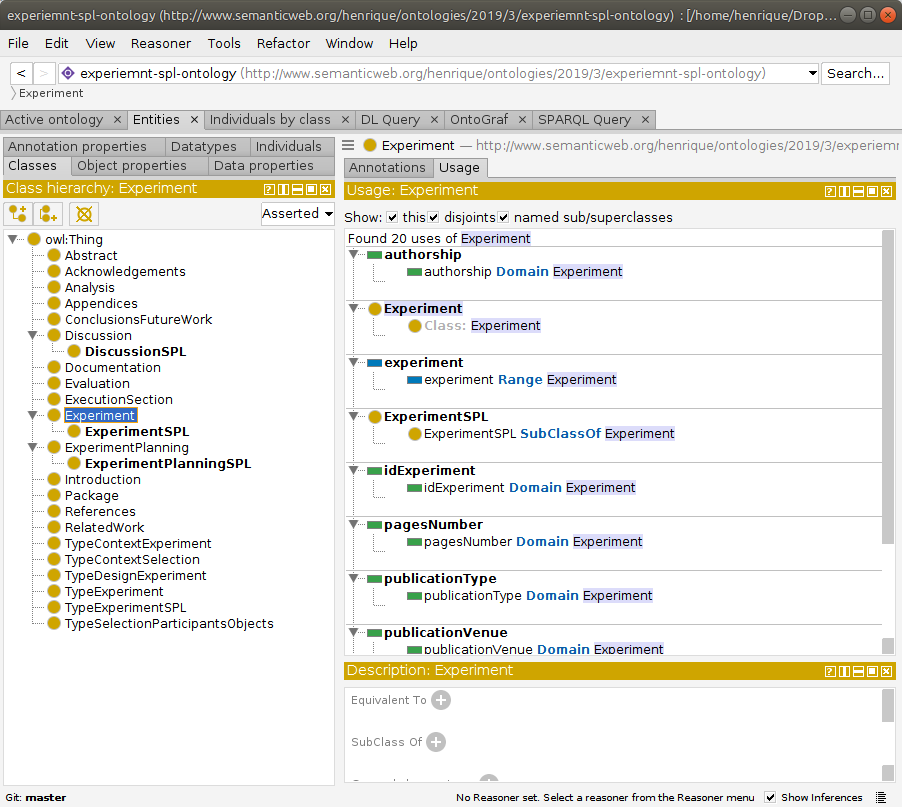
\includegraphics[scale=.3]{entidades-protege.png}
	\caption{Definição da classe Experiment no Protégé.}
	\label{figure:class_defition_protege}
\end{figure}

\subsubsection{Definição das propriedades de objetos}
No Protégé, definimos uma propriedade de objeto raiz chamada topObjectProperty na qual todas as outras propriedades são filhas dela. A \ref{figure:object_prop_defition_protege} Figura apresenta a definição de propriedade de objeto para chamada ?documentation? dentro do modelo, neste momento a definição é composta pelo nome da propriedade e seus relacionamentos com classes, Domains e Ranges.

\begin{figure}[htb]
	\centering 
	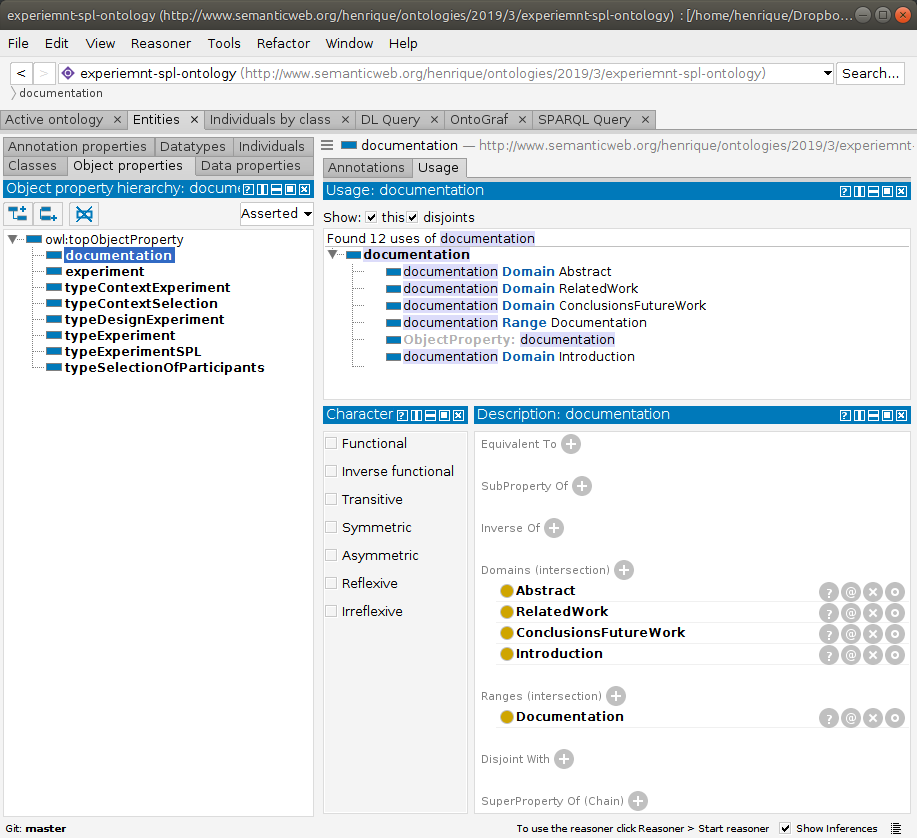
\includegraphics[width=10cm]{entidades-protege-object-properties.png}
	\caption{Definição da propriedade de objeto documentation no Protégé.}
	\label{figure:object_prop_defition_protege}
\end{figure}

\subsubsection{Definição das propriedades dos dados}
No Protégé, definimos uma propriedade de dados raiz chamada topDataProperty na qual todas as outras propriedades são filhas dela. Para cada Propriedade de Dado definimos um conjunto de classes de seu Domínio e um conjunto de tipos de dados (predefinido) de seu Alcance, por exemplo, a propriedade de dado ?nameSPLUsed? possui como classe de domínio ExperimentSPL e como alcance um xsd:string. A \ref{figure:data_prop_defition_protege} apresenta a definição de propriedade de dado para chamada ?nameSPLUsed? dentro do modelo, neste momento a definição é composta pelo nome da propriedade e seus relacionamentos, Domains (uma classe) e Ranges (uma tipagem).

\begin{figure}[htb]
	\centering 
	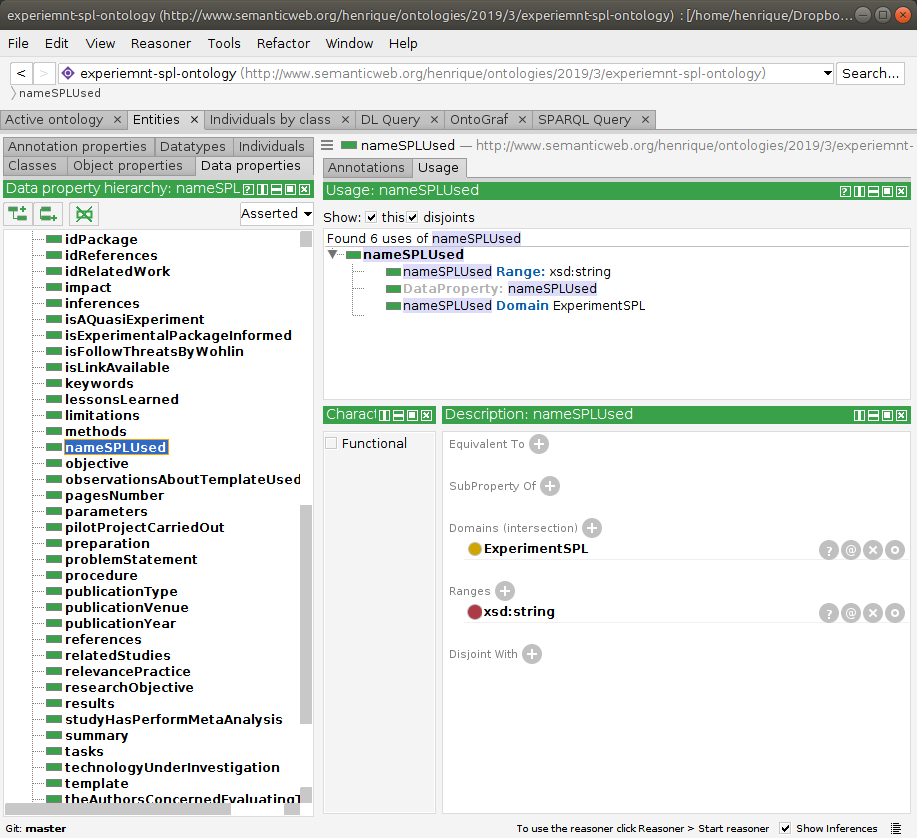
\includegraphics[width=10cm]{entidades-protege-data-properties.png}
	\caption{Definição da propriedade de dado nameSPLUsed no Protégé.}
	\label{figure:data_prop_defition_protege}
\end{figure}

\subsubsection{Artefato gerado pelo Protégé}

Ao final, o Protégé gera um arquivo .owl contendo a definição do modelo. A \ref{figure:graph_ontology_model} fornece uma visão geral do formato do grafo do projeto, contendo todas as classes e suas propriedades de objeto e propriedade de dados. Usamos a ferramenta WebVOWL \cite{lohmann2016visualizing} para gerar essa visão.

\begin{figure}[htb]
	\centering 
	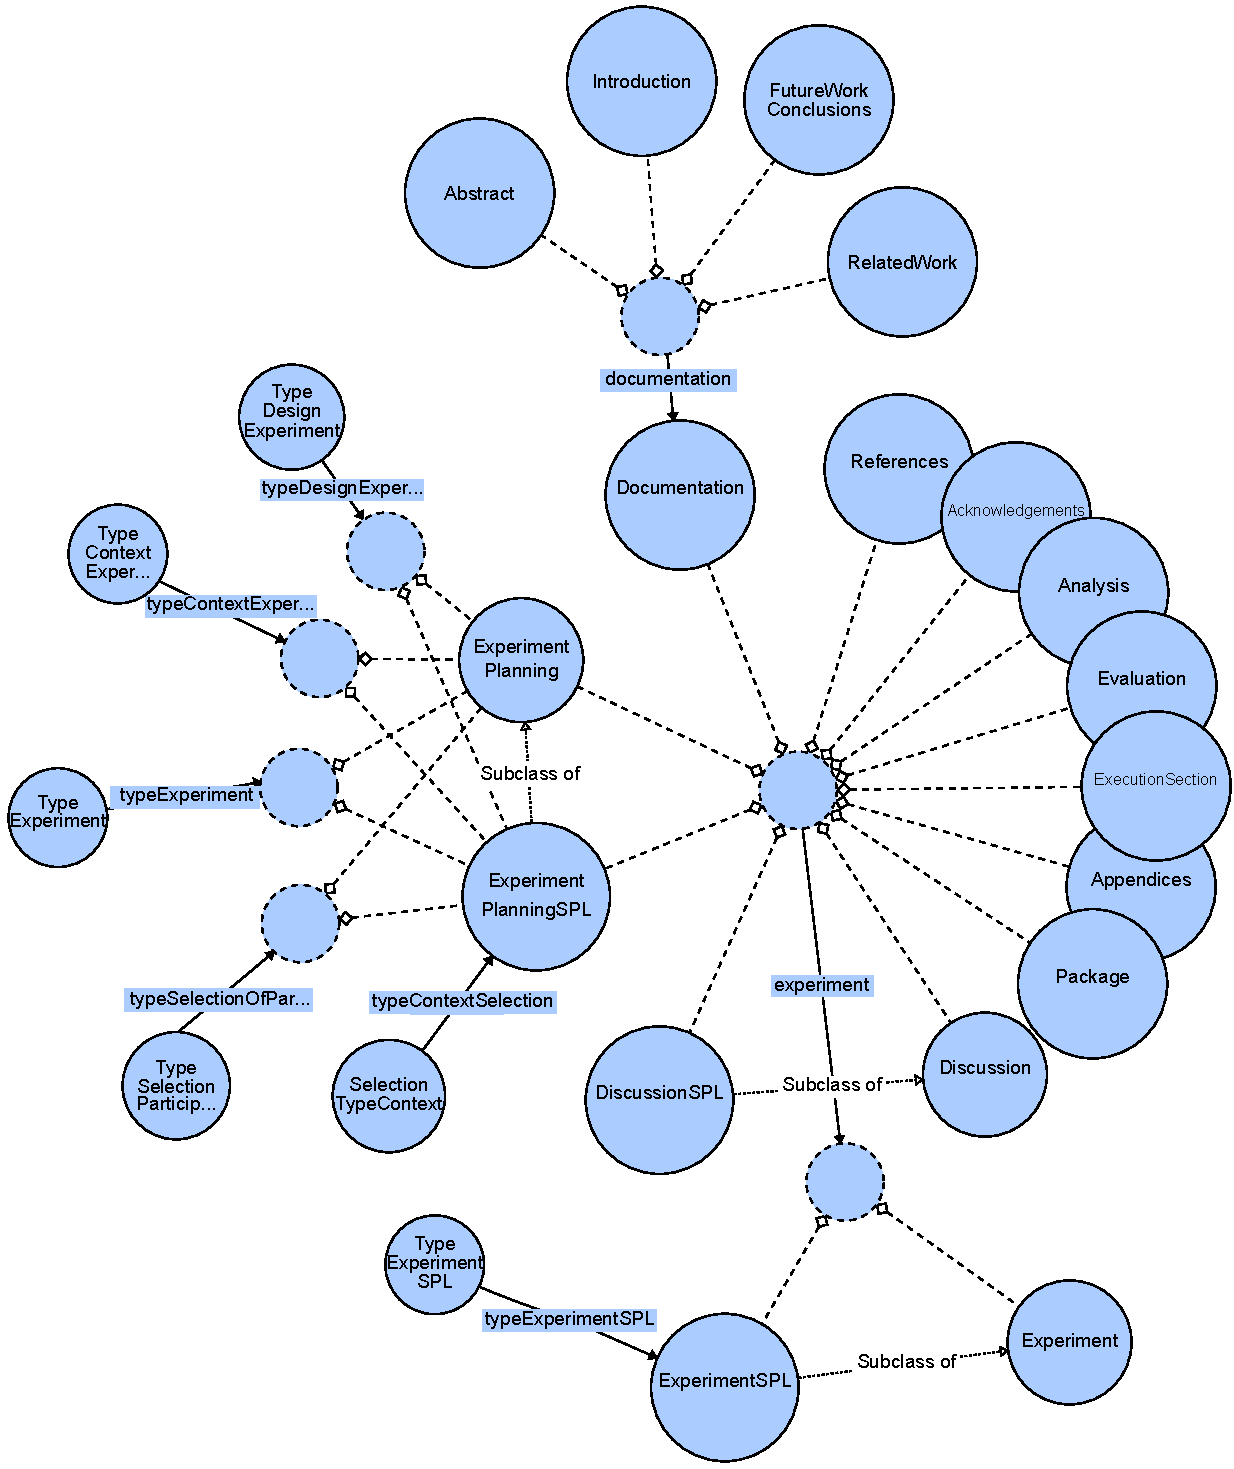
\includegraphics[width=10cm]{ontology-populate-valid-owl-2.pdf}
	\caption{Grafo da modelagem da ontologia - gerado pelo WbVOWL.}
	\label{figure:graph_ontology_model}
\end{figure}

\subsection{Pyton}
\label{sec:python}

A próxima etapa, após a modelagem da ontologia, foi inserir os indivíduos na mesma, ou seja, popular a ontologia para realização de inferências futuras. Apesar do Protégé ter capacidade para realizar essa operação, optamos por utilizar um script para realizar tal tarefa, visto que, no Protégé o processo de inserir indivíduos na ontologia é realizado de modo manual, por meio do menu ?Individuals by Class?, onde é preciso selecionar propriedade por propriedade para cada indivíduo. Sabendo que para cada indivíduo temos 84 propriedades de dados mais 8 propriedade de objetos, somando um total de 92 relacionamentos para cada indivíduo. Portanto, sabendo que temos 174 indivíduos a serem inseridos em uma carga inicial, seriam mais de 16000 iterações manuais no Protégé.

Dado essa estimativa de operações manuais optamos pela utilização de uma ferramenta script a fim de facilitar e automatizar a inserção dos indivíduos e posteriormente a inserção de novos indivíduos. Escolhemos a linguagem de programação Python por fornecer bibliotecas prontas, tanto para manipulação de dados em planilhas (Pandas), como para ontologia em arquivos .owl (OwlReady2).

\subsubsection{Script}

Para criação do script utilizamos outra ferramenta do Python chamada Jupyter Notebook \cite{PER-GRA:2007} para auxiliar na execução e validação de código. O processo do script se assemelha a um processo de ETL (Extract Transform Load), onde extraímos os dados originais da planilha, desenvolvida no trabalho de revisão sistemática sobre experimentos em LPS, e manipulamos estes dados para inserir na ontologia, seguindo a modelagem inicial construída no Protégé.

Para  leitura dos dados da planilha usamos a biblioteca Pandas \cite{mckinney-proc-scipy-2010}, ela nos retorna um objeto do tipo Dataframe que chamamos de ?df?, no qual é a representação da própria planilha no ambiente de programação Python.

Os dados da planilha estão estruturados na seguinte forma, cada linha representa um artigo encontrado no mapeamento sistemático, e cada coluna representa um dado extraído deste artigo. Segue o mapeamento de cada dado. 

Com relação ao Experimento temos:  ID,  Title, Authorship, Publication year, Publication type, Publication venue, Pages number, dados de Experimentos em SPL temos: Is it Real or Academic SPL?, SPL Name used, Was the SPL source used informed? (Y/N) (If yes, which one?). 

Com relação a Documentation temos: Does it use template? (Y/N)?,  If yes, what template?, Observations about the template used. Para o Abstract temos: Objective (What is the question addressed with this research?), Abstract - Background (Why is this research important?), Methods (What is the statistical context and methods applied?), Results (What are the main findings? Practical implications?), Limitations (What are the weakness of this research?), Conclusions (What is the conclusion?) e Keywords. Para o Introduction Section temos: Problem statement (What is the problem? Where does it occur? Who has observed it? Why is it important to be solved?), Research objective (GQM) (What is the research question to be answered by this study?), Context (What information is necessary to understand whether the research relates to a specific situation (environment)?). Para o Related Work Section temos: Technology under investigation (What is necessary for a reader to know about the tecnology to reproduce its application?), Alternative technologies (How does this research relate to alternative technologies? What is the control treatment?), Related studies (How this research relates to existing research (studies)? What were the results from these studies?), Relevance to practice (How does it relate to state of the practice?). Para o Conclusions and Future Work Section temos: Summary (The purpose of this section is to provide a concise summary of the research and its results as presented in the former sections), Impact (Description of impacts with regard to cost, schedule, and quality, circumstances under which the approarch presumably will not yield the expected benefit), Future Work (What other experiments could be run to further investigate the results yielded or evolve the Body of Knowledge).

Com relação ao Experiment Planning temos: Goals (Formalization of goals, refine the important constructs of the experiment's goal), Experimental Units (From which population will the sample be drawn? How will the groups be formed (assignment to treatments)? Any kind of randomization and blinding has to be described?), Experimental Material (Which objects are selected and why?), Tasks (Which tasks have to be performed by the subjects?), Hypotheses (What are the constructs and their operationalization? They have to be traceable derived from the research question respectively the goal of the experiment), Parameters (What are the constructs and their operationalization? They have to be traceable derived from the research question respectively the goal of the experiment), Variables (What are the constructs and their operationalization? They have to be traceable derived from the research question respectively the goal of the experiment), Experiment Design (What type of expimental design has been chosen?), Procedure (How will the experiment (i.e., data collection) be performed? What instruments, materials, tools will be used and how?) Analysis Procedure (How will the data be analyzed?), Is it a quasi-experiment? (Y/N) If yes, is it explicit in the study?, Is it an Original or Replicated Experiment?,	How was the selection of participants/experimental objects? - Simple random sampling; - Systematic sampling; - Stratified random sampling; - Convenience sampling; - Quota sampling, Context of the experiment (in vivo, in vitro, ...), Design Experimental: - One factor with two treatments; - One factor with more than two treatments; - Two factors with two treatments; - More than two factors each with two treatments, SPL artifact used, Context Selection (Off-line vs. on-line, Student vs. professional, Toy vs. real problems, Specific vs. general).

Com relação a Execution (Operation) temos: Preparation (What has been done to prepare the execution of the experiment (i.e., schedule, training), Deviations from the Plan (Describe any deviations from the plan, e.g., how was the data collection actually performed?), The pilot project was carried out? (Y/N) If Yes, how many?

Com relação a Analysis (Analysis and Interpretation) temos: Descriptive statistics (What are the results from descriptive statistics?), Data set preparation (What was done to prepare the data set, why, and how?), Hypothesis testing (How was the data evaluated and was the analysis model validated?), Do it have qualitative analysis of the experiment? (Y/N), If yes, what qualitative analysis was performed?, How the data has been analyzed? (Ex: Correlation, Hypothesis Test, meta-analysis), Is the conclusion of the experiment analysis based on P-value? (Y/N), Did the study perform meta-analysis? (Y/N).

Com relação a Discussion temos: Evaluation of Results and Implications (Explain the results and the relation of the results to earlier research, especially those mentioned in the Background section), Threats to Validity (How is validity of the experimental results assured? How was the data actually validated?) (Follow are the 4 threats proposed by Wohlin: internal, external, construct and conclusion? (Y/N)), Inferences (Inferences drawn from the data to more general conditions), Lessons learned (Which experience was collected during the course of the experiment), Threats to validity in SPL.

Com relação a Evaluation temos: The authors were concerned with evaluating the quality of the experiments? (Y/N)

Com relação a Package temos: Is the experimental package informed? (Y/N) (If yes, what URL? And the link is still available? (Y/N))

Outros dados: Acknowledgements Section (Sponsors, participants, and contributors who do not fullfit the requirements for authorship should be mentioned), References Section (All cited literature has to be presented in the format requested by the publisher, Appendices Section (Experimental materials, raw data, and detailed analyses, which might be helpful for others to build upon the reported work should be provided)

\subsubsection{Manipulação dos Dados}

Para inserir os indivíduos na SMartyOntology, foi preciso manipular os dados da planilha com as seguintes operações.

Primeira operação, split de dados de uma única coluna para duas propriedades de dados da ontologia. Este caso ocorreu para os seguintes dados, as propriedades e prefixadas com ?\_? foram tratadas no próximo passo:

\begin{itemize}
	\item ?Was the SPL source used informed? (Y/N) (If yes, which one?)? para \_informedSPL e sourceSPL;
	\item ?The pilot project was carried out? (Y/N) If Yes, how many?? para \_hasPilot e \_howManyPilot;
	\item ?Is it a quasi-experiment? (Y/N) If yes, is it explicit in the study?? para \_hasQuasiExperiment e quasiExperiment;
	\item ?'Threats to Validity (How is validity of the experimental results assured? 'How was the data actually validated?) (Follow are the 4 threats proposed by Wohlin: internal, external, construct and conclusion? (Y/N)))? para \_hasThreatsValidityByWolin e threatsValidity.
\end{itemize}

Segunda operação, transformação de dados booleanos, strings vazias e números. Foi desenvolvido tres funções de conversão, (i) convertToBoolean, (ii) convertStringEmpty e (iii) convertToNumber. Este caso ocorreu para os seguintes dados:

\begin{itemize}
	\item ?Does it use template? (Y/N)?? para useTemplate aplicando o método convertToBoolean;
	\item ?If yes, what template?? para template aplicando o método convertStringEmpty;
	\item ?Do it have qualitative analysis of the experiment? (Y/N)? para hasQualitativeAnalysis aplicando o método convertToBoolean;
	\item ?Did the study perform meta-analysis? (Y/N)? para hasMetaAnalysis aplicando o método convertToBoolean;
	\item \_informedSPL para informedSPL aplicando o método convertToBoolean;
	\item \_hasQuasiExperiment para hasAQuasiExperiment aplicando o método convertToBoolean;
	\item \_hasPilot para hasPilot aplicando o método convertToBoolean;
	\item \_howManyPilot para howManyPilot aplicando o método convertToNumber;
	\item \_hasThreatsValidityByWolin para hasThreatsValidityByWolin aplicando o método convertToBoolean;
	\item \_hasPackage para hasExperimentalPackage aplicando o método convertToBoolean;
\end{itemize}

Terceira operação, separação do conjunto de dados com informação explícita de SPL. Separamos o conjunto total de 174 artigos em artigos de experimentos que contêm informações explícitas de SPL (152) e artigos que não contêm informação explícitas de SPL (22), para criação dos indivíduos conforme as classes modeladas na ontologia com atributos pertinentes a SPL.

Quarta operação, padronização de dados constantes e faltantes. Foi preciso padronizar os dados em casos faltantes foi atribuído um padrão. Isso ocorreu para os seguintes dados:

\begin{itemize}
	\item "Is it Real or Academic SPL?" foi definido o seguinte conjunto de dados [REAL, ACADEMY] sendo o padrão "ACADEMY";
	\item "Is it an Original or Replicated Experiment?" foi definido o seguinte conjunto de dados [ORIGINAL, REPLICATED] sendo o padrão "REPLICATED"
	\item "How was the selection of participants/experimental objects? - Simple random sampling; - Systematic sampling; - Stratified random sampling; - Convenience sampling; - Quota sampling." foi definido o seguinte conjunto de dados [SIMPLE\_RANDOM\_SAMPLING, SYSTEMATIC\_SAMPLING, STRATIFIED\_RANDOM\_SAMPLING,	CONVENIENCE\_SAMPLING, QUOTA\_SAMPLING] sendo o padrão "CONVENIENCE\_SAMPLING";
	\item "Context of the experiment (in vivo, in vitro, ...)" foi definido o seguinte conjunto de dados [IN\_VIVO, IN\_VITRO] sendo o padrão "IN\_VITRO";
	\item "Design Experimental: - One factor with two treatments; - One factor with more than two treatments; - Two factors with two treatments; - More than two factors each with two treatments." foi definido o seguinte conjunto de dados [ONE\_FACTOR\_WITH\_TWO\_TREATMENTS, ONE\_FACTOR\_WITH\_MORE\_THAN\_TWO\_TREATMENTS, TWO\_FACTORS\_WITH\_TWO\_TREATMENTS, MORE\_THAN\_TWO\_FACTORS\_EACH\_WITH\_TWO\_TREATMENTS] sendo o padrão "ONE\_FACTOR\_WITH\_TWO\_TREATMENTS";
	\item "Context Selection (Off-line vs. on-line, Student vs. professional, Toy vs. real problems, Specific vs. general)" foi definido o seguinte conjunto de dados [OFFLINE, ONLINE, STUDENT, PROFESSIONAL, TOY, REAL\_PROBLEMS, SPECIFIC, GENERAL] sendoo padrão "GENERAL";
\end{itemize}

\subsubsection{Inserção do indivíduos e criação dos relacionamentos}

Inicialmente fazemos a leitura do modelo da ontologia gerada pelo Protégé (arquivo .owl) por meio da biblioteca Owlready2, com isso temos um objeto chamado ?onto? onde a partir dele podemos executar operações de inserção de indivíduos e outras operações na ontologia no ambiente de programação Python.

O processo de inserção dos dados extraídos da planilha se dá por, percorrer linha a linha da planilha, e criar os indivíduos um a um de cada classe modelada na ontologia com seus respectivos atributos. Para isso foi necessário criar vários métodos a fim de facilitar a compreensão do script.

Foi criado dois laços para percorre os dois subconjuntos de dados, um com informações explícitas de SPL chamado de df\_spl  e outro chamado df\_exp. O primeiro laço sobre df\_spl invoca a seguinte sequencia de métodos: registreExperimentSPL > registreExperimentPlanningSPL > registreDiscussionSPL > registerCommons. O segundo laço sobre df\_exp invoca a seguinte sequencia de métodos: registreExperiment > registreExperimentPlanning > registreDiscussion > registerCommons.

\begin{lstlisting}[language=Python, caption=The first loop on \texttt{df\_spl}, label=lst:first-loop]
for idx, row in df_spl.iterrows():
experimentSPL = registreExperimentSPL(idx, row)

experimentPlanningSPL = registreExperimentPlanningSPL(idx, row)
experimentPlanningSPL.experiment.append(experimentSPL)

discussion = registreDiscussionSPL(idx, row)
discussion.experiment.append(experimentSPL)

registerCommons(experimentSPL, idx, row)
\end{lstlisting}

\begin{lstlisting}[language=Python, caption=The second loop on \texttt{df\_exp}, label=lst:second-loop]
for idx, row in df_exp.iterrows():
experiment = registreExperiment(idx, row)

experimentPlanning = registreExperimentPlanning(idx, row)
experimentPlanning.experiment.append(experiment)

discussion = registreDiscussion(idx, row)
discussion.experiment.append(experiment)

registerCommons(experiment, idx, row)
\end{lstlisting}

O método registreExperimentSPL executa o método registreExperimentCommons e retorna uma instância de indivíduo da ontologia da classe onto.ExperimentSPL.

O método registreExperiment executa o método registreExperimentCommons e retorna uma instância de indivíduo da ontologia da classe onto.Experiment.

O método registreExperimentCommons recebe uma instância tanto de onto.ExperimentSPL ou onto.Experiment e atribui as variáveis comuns para ambas as classes.

O método registreExperimentPlanningSPL executa o método registreExperimentPlanningCommons e retorna uma instância de indivíduo da ontologia da classe onto.ExperimentPlanningSPL.

O método registreExperimentPlanning executa o método registreExperimentPlanningCommons e retorna uma instância de indivíduo da ontologia da classe onto.ExperimentPlanning.

O método registreExperimentPlanningCommons recebe uma instância tanto de onto.ExperimentPlanningSPL ou onto.ExperimentPlanning e atribui as variáveis comuns para ambas as classes.

O método registreDiscussionSPL executa o método registreDiscussionCommons e retorna uma instância de indivíduo da ontologia da classe onto.DiscussionSPL.

O método registreDiscussion executa o método registreDiscussionCommons e retorna uma instância de indivíduo da ontologia da classe onto.Discussion.

O método registreDiscussionCommons recebe uma instância tanto de onto.DiscussionSPL ou onto.Discussion e atribui as variáveis comuns para ambas as classes.

O método registerCommons que recebe uma instância tanto de onto.ExperimentSPL ou onto.Experiment e executa a sequência de métodos:  registreDocumentation - que retorna uma instância de onto.Documentation e atribui a instância de experiment a ela > registreAbstract - que retorna uma instância de onto.Abstract e atribui a instância de documentation a ela > registreIntroduction - que retorna uma instância de onto.Introduction e atribui a instância de documentation a ela > registreRelatedWork - que retorna uma instância de onto.RelatedWork e atribui a instância de documentation a ela > registreConclusionsFutureWork - que retorna uma instância de onto.ConclusionsFutureWork e atribui a instância de documentation a ela > registreExecutionSection - que retorna uma instância de onto.ExecutionSection e atribui a instância de experiment a ela > registreAnalysis - que retorna uma instância de onto.Analysis e atribui a instância de experiment a ela > registreAcknowledgements - que retorna uma instância de onto.Acknowledgements e atribui a instância de experiment a ela > registreReferences - que retorna uma instância de onto.References e atribui a instância de experiment a ela > registreAppendices - que retorna uma instância de onto.Appendices e atribui a instância de experiment a ela > registreEvaluation - que retorna uma instância de onto.Evaluation e atribui a instância de experiment a ela > registrePackage - que retorna uma instância de onto.Package e atribui a instância de experiment a ela.

\subsubsection{Artefato e validação}
Ao final dos dois laços temos o objeto ?onto? populado com com os indivíduos, e por meio da biblioteca Owlready2 geramos um novo arquivo .owl contendo a modelagem da ontologia mais a população de indivíduos. O arquivo da modelagem inicial contém 66,3 kB, e o arquivo populado contém 4,8 MB.

No final do script tem existe um passo de validação onde conferimos a quantidade de linhas da planilha com a quantidade de indivíduos inserido na ontologia, pode ser visto em \ref{lst:stap-validation}.

\begin{lstlisting}[language=Python, caption=Stap validation, label=lst:stap-validation]
assert len (onto.Experiment.instances ()) == df.shape [0]
\end{lstlisting}

\section{Exemplo de Aplicação}
\label{sec:exemplo}

Foi criado também um exemplo de recomendação com a seguinte questão de recomendação, ?Qual artefato de SPL usar dos experimentos que usam a mesma template experimental mais recorrente?. Com base nesta questão foi criado um script Python utilizando as bibliotecas Pandas e OwlReady2, para responder a mesma.

O script começa carregando a ontologia preenchida e, em seguida, executamos a consulta SPARQL \ref{code:...} para retornar os agrupados pela template experimental, estes indivíduos são do tipo Documentation. Na sequência, filtramos da lista inicial de indivíduos que usam modelos, aqueles que usam o modelo mais recorrente. Com esses indivíduos em mãos, buscamos seu relacionamento com indivíduos do tipo ExperimentPlanningSPL para extrair informações de artefatos de SPL. Assim, podemos recomendar qual artefato de SPL, com base no artefato mais usado desses indivíduos filtrados.

O script começa carregando a ontologia povoada, e em seguida extrai os indivíduos que usam template experimental, estes indivíduos são do tipo Documentation. Atribuímos este resultado a um objeto do tipo Pandas para executar a função .values\_counts() que retorna o agrupamento somado das templates mais usadas. Na sequência, filtramos da lista inicial dos indivíduos que usam templates, aqueles que usam a template mais recorrente. Com estes indivíduos em mãos, buscamos o relacionamento deles com os indivíduos do tipo ExperimentPlanningSPL para extrair a informação dos artefatos de SPL. Então podemos recomendar qual artefato de SPL, com base no artefato mais usado destes individuos filtrados.

\begin{figure}[ht]
 	\centering 
 	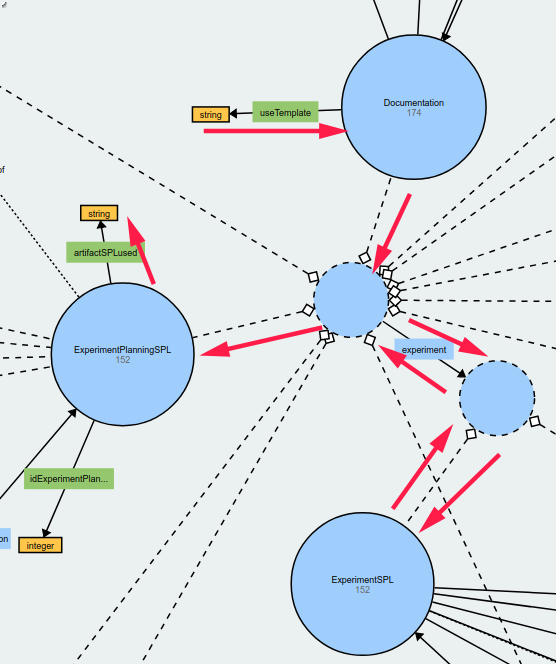
\includegraphics[width=6.5cm]{filter-in-ontology-path.png}
 	\caption{Graph Path to Recommendation Example.}
 	\label{figure:graph_path_to_recomendation}
 \end{figure}

O grafo da \ref{figure:graph_path_to_recomendation} mostra o caminho percorrido entre as classes e propriedades de objetos e dados para chegar no artefato de SPL a ser recomendado.

O exemplo de recomendação apresenta como podemos criar mecanismos de inferência no modelo de ontologia proposto neste trabalho. Foi possível avaliar que com algumas consultas e verificações é possível extrair informações e meta informações sobre experimentos em SPL. 

Este exemplo percorre três classes (Documentation, ExperimentSPL e ExperimentPlanningSPL) de 24 classes, duas propriedades de objetos (documentation e experimet) de 8 propriedades e três propriedades de dados (useTemplate, template e artifactSPLused) de 87 propriedades de dados do modelo proposto. O cálculo . estima que neste exemplo estamos usando 0,1% da capacidade de resposta que o modelo possa responder.

%uso de classe * %uso de propriedade de objeto * %uso de propriedade de dados = %uso da ontologia.

O exemplo apresenta como podemos criar mecanismos de inferência no modelo de ontologia proposto neste trabalho. Foi possível avaliar que com algumas consultas e verificações é possível extrair informações e meta informações sobre experimentos em SPL. 

Este exemplo percorre três classes (Documentation, ExperimentSPL e ExperimentPlanningSPL) de 24 classes, duas propriedades de objetos (documentation e experimet) de 8 propriedades e três propriedades de dados (useTemplate, template e artifactSPLused) de 87 propriedades de dados do modelo proposto. O cálculo . estima que neste exemplo estamos usando 0,1\% da capacidade de resposta que o modelo possa responder.

%uso de classe * %uso de propriedade de objeto * %uso de propriedade de dados = %uso da ontologia.

%****CÁLCULO DO USO ESTIMADO DA ONTOLOGIA*** POSSIBILIDADES DE CAMINHOS ENTRE CLASSES E PROPRIEDADES.

No caso do exemplo de recomendação a primeira parte do retorna a template mais recorrente. O resultado é a saída do script: ?Template more frequency is Wohlin? seguida da Fig. que representa os dados da Tabela.

E segunda parte encontra qual artefato de SPL dos indivíduos que usam a template encontrada na primeira etapa. o resultado é a saída do script: ?Artifact more used is the "test cases" to template: Wohlin? seguido da Fig.

\section{Avaliação Empírica}
\label{sec:avaliacao}

Para avaliação da ontologia seguimos duas estratégias, uma para avaliar possíveis armadilhas e falhas no modelo de ontologia proposto.

Usamos a ferramenta OOPS! para gerar avaliação do modelo de ontologia proposto. A ferramenta ajuda a detectar algumas das armadilhas mais comuns que aparecem ao desenvolver ontologias [referência].

\begin{itemize}
	\item P01. Criando elementos polissêmicos;
	\item P02. Criando sinônimos como classes;
	\item P03. Criando o relacionamento `` is '' em vez de usar `` rdfs: subClassOf ''; `` rdf: type '' ou `` owl: sameAs '';
	\item P04. Criando elementos de ontologia não conectados;
	\item P05. Definindo relações inversas erradas;
	\item P06. Incluindo ciclos em uma hierarquia de classes;
	\item P07. Mesclar diferentes conceitos na mesma classe;
	\item P08. Anotações ausentes;
	\item P09. Informações de domínio ausentes;
	\item P10. Desarticulação em falta;
	\item P11. Domínio ou intervalo ausente nas propriedades;
	\item P12. Propriedades equivalentes não explicitamente declaradas;
	\item P13. Relações inversas não explicitamente declaradas;
	\item P14. Uso indevido de `` owl: allValuesFrom '';
	\item P15. Usando `` alguns não '' no lugar de `` não alguns '';
	\item P16. Usando uma classe primitiva no lugar de uma definida;
	\item P17. Superespecialização de uma hierarquia;
	\item P18. Superespecialização do domínio ou intervalo;
	\item P19. Definir vários domínios ou intervalos nas propriedades;
	\item P20. Uso indevido de anotações de ontologia;
	\item P21. Usando uma classe diversa;
	\item P22. Usando diferentes convenções de nomenclatura na ontologia;
	\item P23. Duplicando um tipo de dados já fornecido pela linguagem de implementação;
	\item P24. Usando definições recursivas;
	\item P25. Definir um relacionamento como inverso de si mesmo;
	\item P26. Definindo relações inversas para uma simétrica;
	\item P27. Definir propriedades equivalentes erradas;
	\item P28. Definindo relacionamentos simétricos errados;
	\item P29. Definindo relacionamentos transitivos errados;
	\item P30. Classes equivalentes não explicitamente declaradas;
	\item P31. Definir classes equivalentes erradas;
	\item P32. Várias aulas com o mesmo rótulo;
	\item P33. Criando uma cadeia de propriedades com apenas uma propriedade;
	\item P34. Classe sem tipografia;
	\item P35. Propriedade não tipificada;
	\item P36. URI contém extensão de arquivo;
	\item P37. Ontologia não disponível na Web;
	\item P38. Nenhuma declaração de ontologia OWL;
	\item P39. Namespace ambíguo;
	\item P40. Sequestro de namespace;
	\item P41. Nenhuma licença declarada.
\end{itemize}

Apesar da ferramenta OOPS! ter 41 pontos de avaliação ela executa apenas 34 pontos semi-automaticamente, pois os outros dependem de domínio específico da ontologia e eles encorajam os usuários a melhorarem a ferramenta. O resultado dado pela ferramenta sugere como os elementos da ontologia poderiam ser modificados para melhorar a qualidade da ontologia. No entanto, nem todas as armadilhas identificadas devem ser interpretadas como erro,, mas como sugestões que devem ser revisadas manualmente em alguns casos. 

Esta avaliação pode ajudar a descobrir erros que foram escondidos por causa da falta de informação. Por exemplo, algumas armadilhas são detectadas pela comparação de domínios e intervalos em propriedades, se não estiverem definidas, as armadilhas não podem ser identificadas. Nesse sentido, corrigindo a armadilha "Falta do domínio ou intervalo em propriedades"  faz com que a ferramenta para encontrar outras armadilhas, por exemplo, ?Definir relações simétricas que não possuem o mesmo domínio e alcance?.

A ferramenta elenca cada armadilha como:

\begin{itemize}
	\item \textbf{Critical}: Corrigir a armadilha é crucial. Caso contrário, isso poderia afetar a consistência, raciocínio, aplicabilidade, etc. da ontologia;
	\item \textbf{Importante}: Embora não seja crítico para a função de ontologia, é importante corrigir este tipo de armadilha;
	\item \textbf{Minor}: Não é realmente um problema, mas ao consertá-lo, tornaremos a ontologia mais agradável.
\end{itemize}

A Tabela. apresenta o resumo do resultado ao rodar nosso modelo de ontologia proposto na ferramenta OOPS!.

\begin{table*}[!ht]
	\caption{Result Summary of the OOPS! evaluation!}
	\label{tab:result_of_evaluation}
	\begin{tabular}{@{}lll@{}}
		\toprule
		\textbf{Pitfall} & \textbf{Description} & \textbf{Critical Level} \\ \midrule
		P08 & \begin{tabular}[c]{@{}l@{}}Missing annotations in 119 cases\end{tabular} & Minor \\
		P10 & \begin{tabular}[c]{@{}l@{}}Missing disjointness on ontology*\end{tabular} & Important \\
		P12 & \begin{tabular}[c]{@{}l@{}}Equivalent properties not explicitly declared in 1 case\end{tabular} & Important \\
		P13 & \begin{tabular}[c]{@{}l@{}}Inverse relationships not explicitly declared in 8 cases\end{tabular} & Minor \\
		P19 & \begin{tabular}[c]{@{}l@{}}Defining multiple domains or ranges in properties in 6 cases\end{tabular} & Critical \\
		P41 & \begin{tabular}[c]{@{}l@{}}No license declared on ontology\end{tabular} & Important \\ \bottomrule
	\end{tabular}
\end{table*}

No caso P08, essa armadilha consiste em criar um elemento de ontologia e não fornecer anotações legíveis a ele. Consequentemente, os elementos de ontologia não possuem propriedades de anotação que os identificam (por exemplo, rdfs: label, lemon: LexicalEntry, skos: prefLabel ou skos: altLabel) ou que os definem (por exemplo, rdfs: comment ou dc: description). Essa armadilha está relacionada às diretrizes fornecidas em [referencia 5 do OOPS].

No caso P10, a ontologia não possui axiomas desarticulados entre classes ou entre propriedades que devem ser definidas como disjuntas. Esta armadilha está relacionada com as orientações fornecidas em [6], [2] e [7].

No caso P12, a ontologia carece de informações sobre propriedades equivalentes (owl: equivalentProperty) nos casos de relacionamentos e / ou atributos duplicados. Os seguintes atributos podem ser definidos como equivalentes: wasTheSPLSourceUsedInformed e wastheSPLSourceUsedInformed.

No caso P13, essa armadilha aparece quando qualquer relacionamento (exceto aqueles que são definidos como propriedades simétricas usando owl: SymmetricProperty) não tem uma relação inversa (owl: inverseOf) definida dentro da ontologia. Esta armadilha aparece nos seguintes elementos: typeSelectionOfParticipants, typeExperimentSPL, typeExperiment, typeDesignExperiment, typeContextSelection, typeContextExperiment, experiment, documentation 

No caso P19, o domínio ou intervalo (ou ambos) de uma propriedade (relacionamentos e atributos) é definido informando mais de uma instrução rdfs: domain ou rdfs: range. Em OWL vários rdfs: domain ou rdfs: axiomas de alcance são permitidos, mas eles são interpretados como conjunção, sendo, portanto, equivalentes ao constructo owl: intersectionOf. Essa armadilha está relacionada ao erro comum que aparece ao definir domínios e intervalos descritos em [7]. Esta armadilha aparece nos seguintes elementos: documentation, experiment, typeContextExperiment, typeDesignExperiment, typeExperiment, typeSelectionOfParticipants 

No caso P41, os metadados de ontologia omitem informações sobre a licença que se aplica à ontologia.

* Armadilha que se aplica à ontologia em geral, em vez de elementos específicos.

\subsection{Perspectivas de Melhorias}
Dada a análise da ferramenta OOPS! o próximo passo será corrigir as armadilhas apresentada na avaliação e reavaliar a ontologia de modo geral, principalmente os pontos que a ferramenta não está automatizada.

